\section{Anexo A: Esquemas de conexionado de los instrumentos}

\subsection{Ensayos de corrientes de fuga}

\begin{figure}[H]
    \centering
    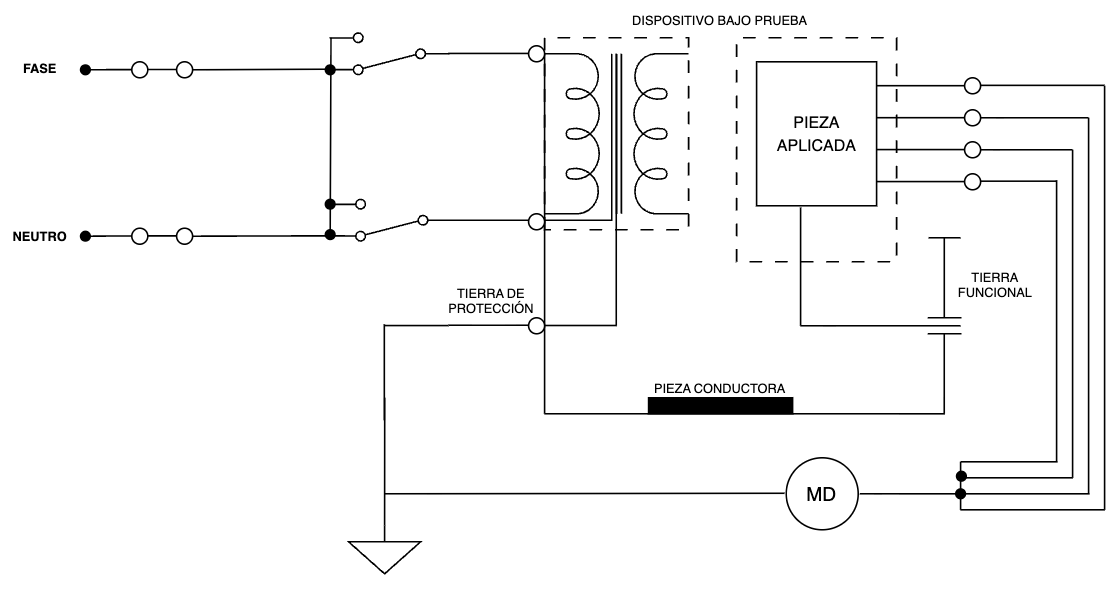
\includegraphics[width=0.75\textwidth]{figuras/Fuga/PA_a_Tierra.png}
    \caption{Ensayo de corriente de fuga de parte aplicada a tierra.}
    \label{fig:fuga_pa_tierra}
\end{figure}

\begin{figure}[H]
    \centering
    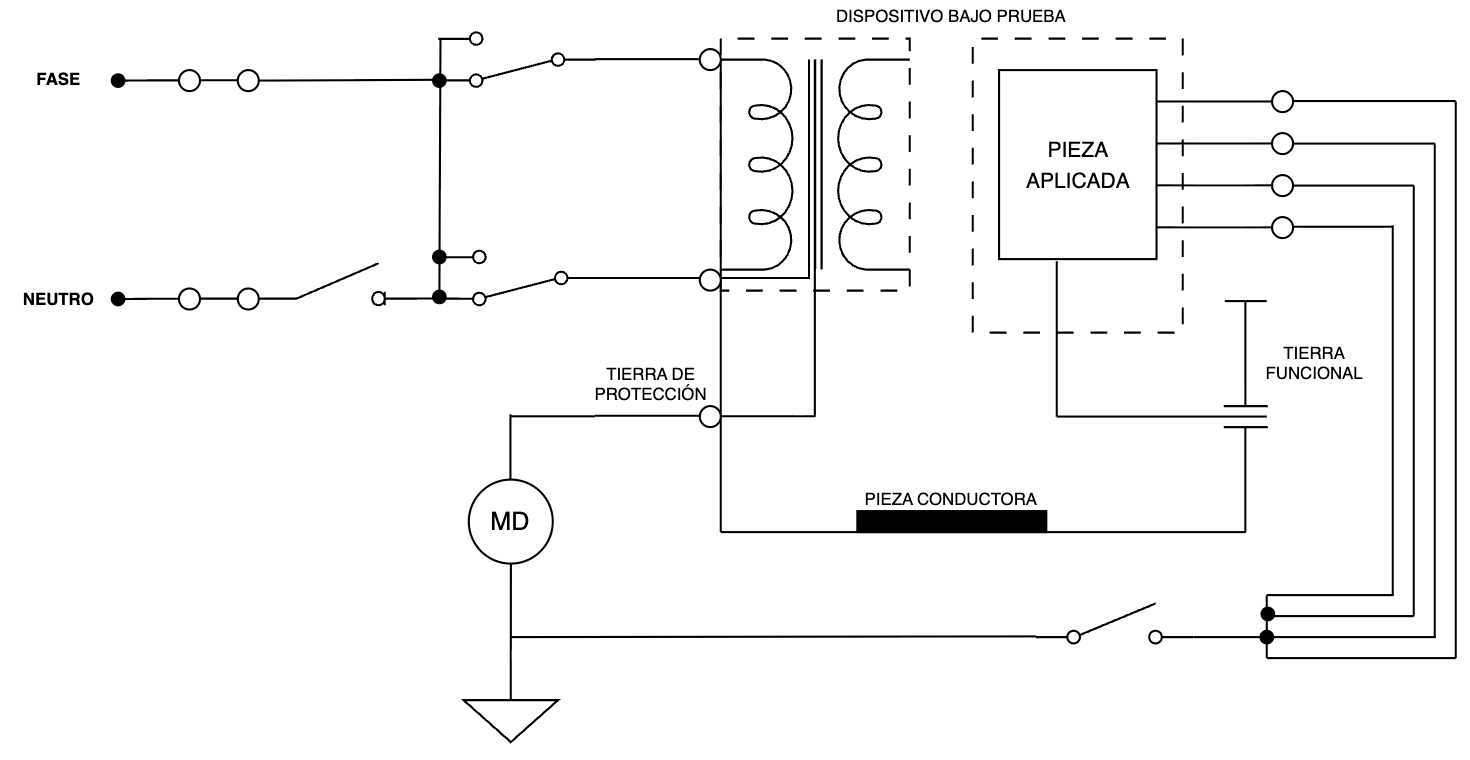
\includegraphics[width=0.75\textwidth]{figuras/Fuga/PE_a_Tierra.png}
    \caption{Ensayo de corriente de fuga de tierra de protección.}
    \label{fig:fuga_pe_tierra}
\end{figure}

\begin{figure}[H]
    \centering
    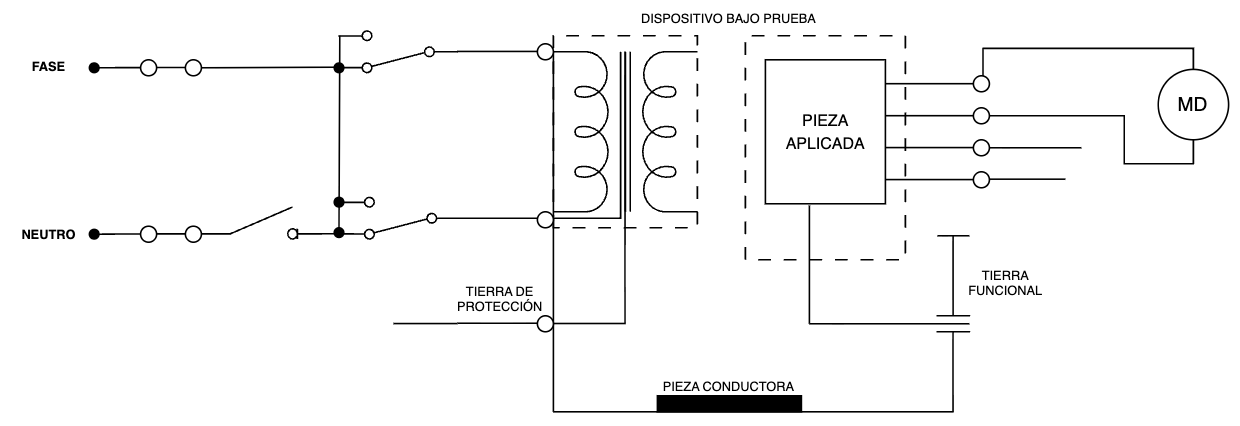
\includegraphics[width=0.75\textwidth]{figuras/Fuga/Entre_PA.png}
    \caption{Ensayo de corriente de fuga entre partes aplicadas.}
    \label{fig:fuga_entre_pa}
\end{figure}

\begin{figure}[H]
    \centering
    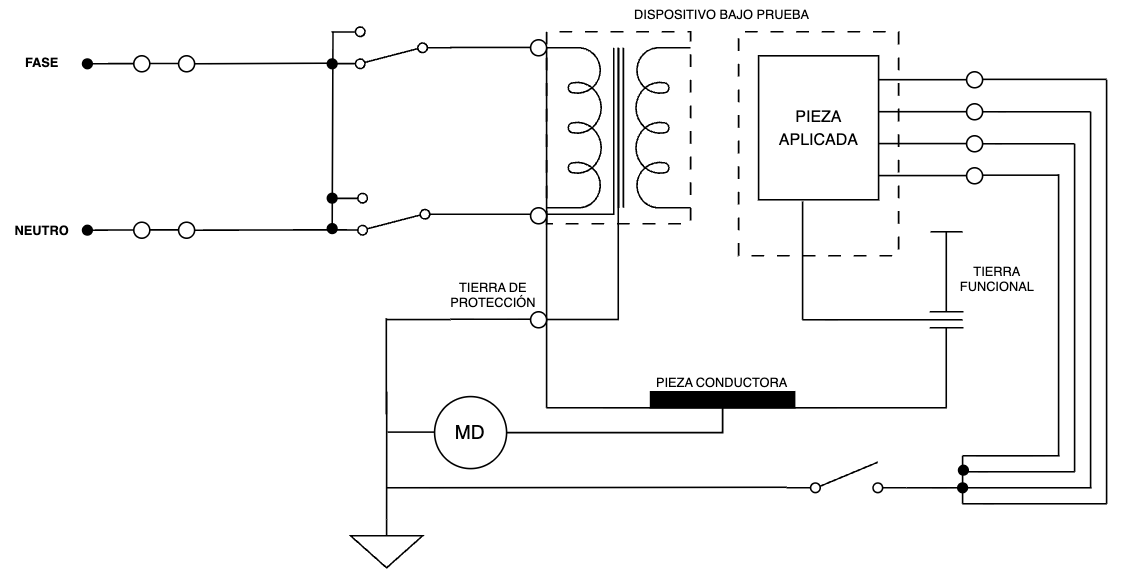
\includegraphics[width=0.75\textwidth]{figuras/Fuga/Carcasa_a_Tierra.png}
    \caption{Ensayo de corriente de fuga entre carcasa y tierra.}
    \label{fig:fuga_carcasa_tierra}
\end{figure}


\subsection{Ensayos de resistencia de aislamiento}

% \begin{figure}[H]
%     \centering
%     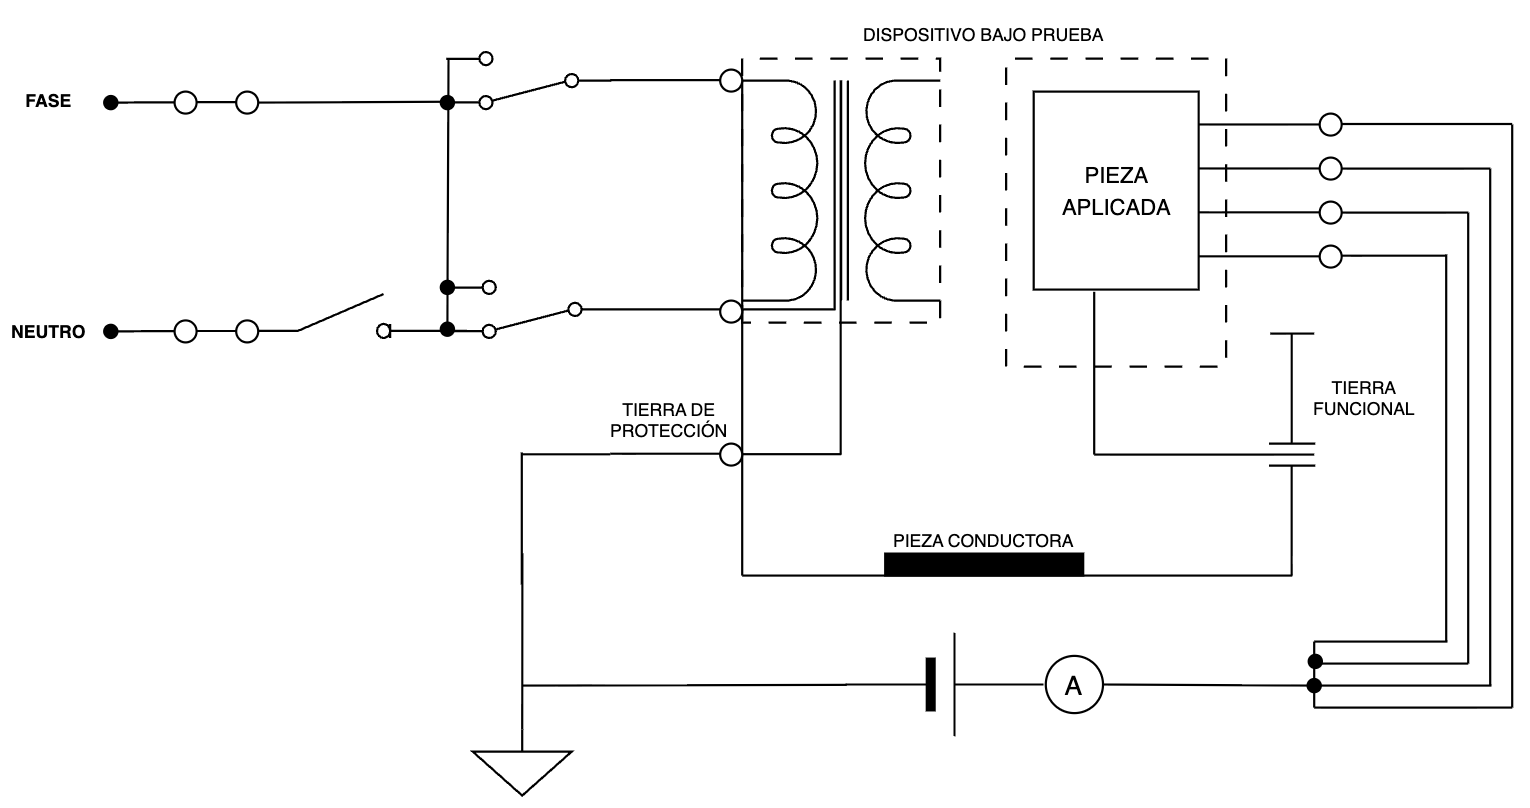
\includegraphics[width=0.75\textwidth]{figuras/Aislamiento/PA_a_PE.png}
%     \caption{Ensayo de resistencia de aislamiento entre parte aplicada y tierra de protección.}
%     \label{fig:aislamiento_pa_pe}
% \end{figure}

\begin{figure}[H]
    \centering
    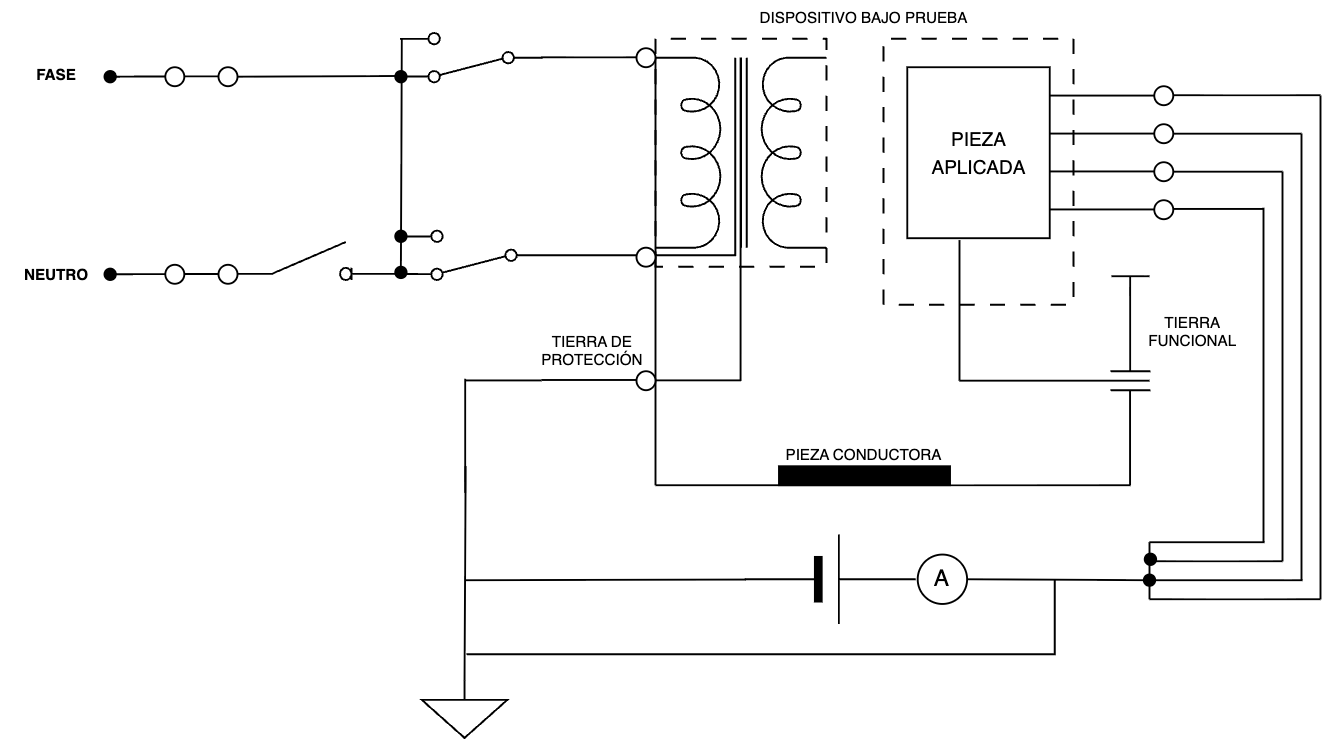
\includegraphics[width=0.75\textwidth]{figuras/Aislamiento/PA_a_PE_v2.png}
    \caption{Ensayo de resistencia de aislamiento entre parte aplicada y tierra de protección.}
    \label{fig:aislamiento_pa_pe_v2}
\end{figure}

\begin{figure}[H]
    \centering
    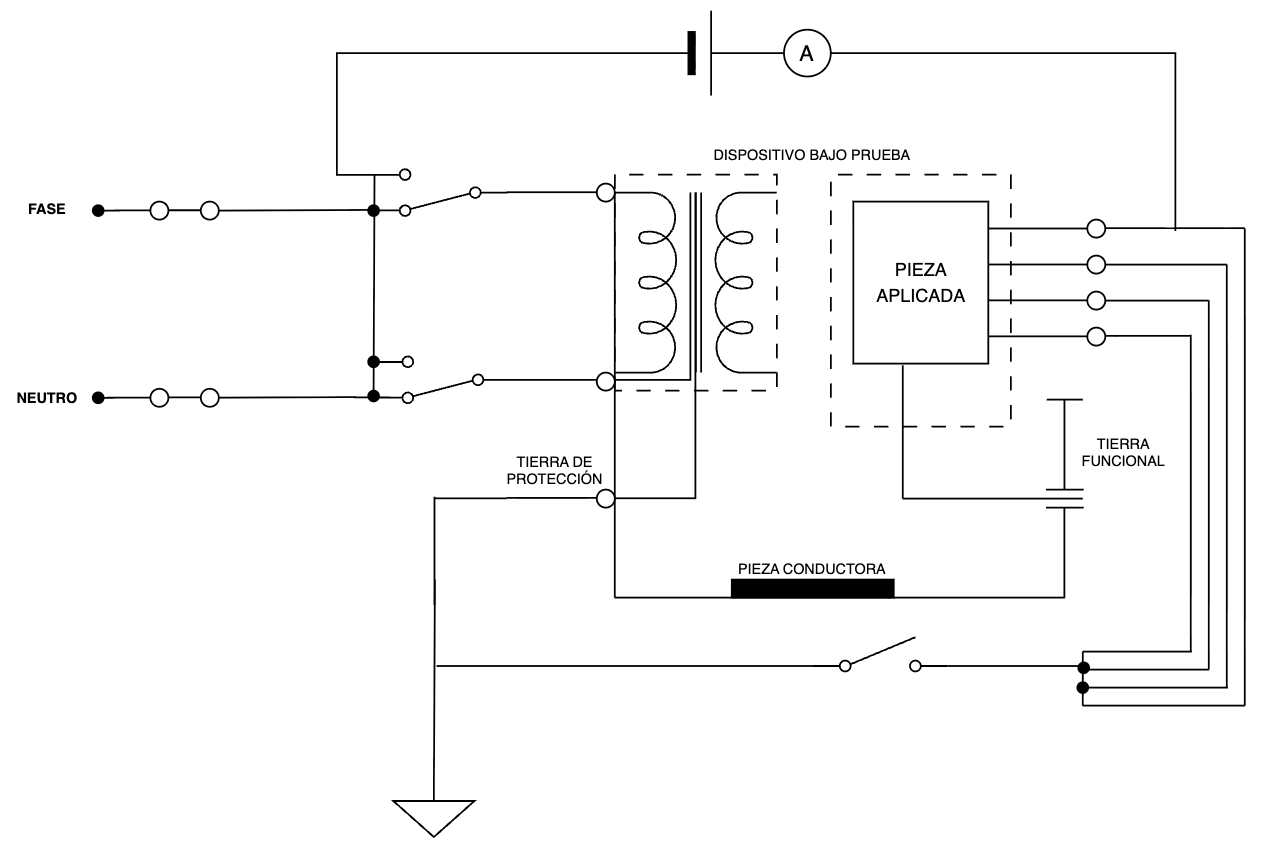
\includegraphics[width=0.75\textwidth]{figuras/Aislamiento/PA_a_Fase.png}
    \caption{Ensayo de resistencia de aislamiento entre parte aplicada y fase.}
    \label{fig:aislamiento_pa_fase}
\end{figure}

\section{Anexo B: Cálculo de la eficiencia de los dispositivos empleados}

\subsection{Medidor de frecuencia cardíaca}
\begin{align*}
\text{Eficacia}_1 &= \left(1 - \frac{|90-91|}{91}\right) \times 100 = 98.90\% \\
\text{Eficacia}_2 &= \left(1 - \frac{|60-60|}{60}\right) \times 100 = 100.00\% \\
\text{Eficacia}_3 &= \left(1 - \frac{|30-30|}{30}\right) \times 100 = 100.00\% \\
\text{Eficacia}_4 &= \left(1 - \frac{|300-300|}{300}\right) \times 100 = 100.00\% \\
\text{Eficacia}_5 &= \left(1 - \frac{|242-240|}{240}\right) \times 100 = 99.17\% \\
\text{Eficacia}_6 &= \left(1 - \frac{|210-210|}{210}\right) \times 100 = 100.00\% \\
\text{Eficacia}_7 &= \left(1 - \frac{|121-120|}{120}\right) \times 100 = 99.17\% \\
\text{Eficacia promedio} &= \frac{98.90 + 100.00 + 100.00 + 100.00 + 99.17 + 100.00 + 99.17}{7} = 99.61\%
\end{align*}

\subsection{Medidor multiparamétrico de saturación de oxígeno y frecuencia cardíaca}
\begin{align*}
\text{Eficacia SpO}_2\text{,}_1 &= \left(1 - \frac{|98-97|}{97}\right) \times 100 = 98.97\% \\
\text{Eficacia SpO}_2\text{,}_2 &= \left(1 - \frac{|75-75|}{75}\right) \times 100 = 100.00\% \\
\text{Eficacia SpO}_2\text{,}_3 &= \left(1 - \frac{|80-80|}{80}\right) \times 100 = 100.00\% \\
\text{Eficacia SpO}_2\text{,}_4 &= \left(1 - \frac{|85-85|}{85}\right) \times 100 = 100.00\% \\
\text{Eficacia SpO}_2\text{ promedio} &= \frac{98.97 + 100.00 + 100.00 + 100.00}{4} = 99.74\% \\[10pt]
\text{Eficacia Frec}_1 &= \left(1 - \frac{|80-80|}{80}\right) \times 100 = 100.00\% \\
\text{Eficacia Frec}_2 &= \left(1 - \frac{|60-60|}{60}\right) \times 100 = 100.00\% \\
\text{Eficacia Frec}_3 &= \left(1 - \frac{|61-60|}{60}\right) \times 100 = 98.33\% \\
\text{Eficacia Frec}_4 &= \left(1 - \frac{|100-100|}{100}\right) \times 100 = 100.00\% \\
\text{Eficacia Frec promedio} &= \frac{100.00 + 100.00 + 98.33 + 100.00}{4} = 99.58\%
\end{align*}

\subsection{Medidor de saturación de oxígeno y frecuencia con oxímetro de pulso}
\begin{align*}
\text{Eficacia SpO}_2\text{,}_1 &= \left(1 - \frac{|91-90|}{90}\right) \times 100 = 98.89\% \\
\text{Eficacia SpO}_2\text{,}_2 &= \left(1 - \frac{|80-80|}{80}\right) \times 100 = 100.00\% \\
\text{Eficacia SpO}_2\text{,}_3 &= \left(1 - \frac{|71-70|}{70}\right) \times 100 = 98.57\% \\
\text{Eficacia SpO}_2\text{ promedio} &= \frac{98.89 + 100.00 + 98.57}{3} = 99.15\% \\[10pt]
\text{Eficacia Frec}_1 &= \left(1 - \frac{|80-80|}{80}\right) \times 100 = 100.00\% \\
\text{Eficacia Frec}_2 &= \left(1 - \frac{|100-100|}{100}\right) \times 100 = 100.00\% \\
\text{Eficacia Frec}_3 &= \left(1 - \frac{|80-80|}{80}\right) \times 100 = 100.00\% \\
\text{Eficacia Frec promedio} &= \frac{100.00 + 100.00 + 100.00}{3} = 100.00\%
\end{align*}